%\documentclass[notes,usenames,dvipsnames]{beamer}
%\documentclass[notes]{beamer}       % print frame + notes
%\documentclass[notes=only]{beamer}   % only notes
\documentclass[usenames,dvipsnames]{beamer}             % only frames
\usepackage[outputdir=out]{minted}
\usepackage{pgfpages}
%\setbeameroption{show notes on second screen}
%\setbeameroption{show notes}
%subfigures
\usepackage{caption}
\usepackage{subcaption}

%tables packages
\usepackage{multirow}

% math
\usepackage{amsmath}

% bash command
\usepackage{graphicx}
\usepackage{listings}
% varbatim for ascii figures
\usepackage[T1]{fontenc}
\usepackage[utf8]{inputenc}
%\usepackage{verbatim}
\usepackage{lipsum} % for context
\usepackage{fancyvrb}
\usepackage{varwidth}
\usepackage{circuitikz}
\ctikzset{logic ports=ieee}
\usepackage{listings}
% \lstset{language=[Motorola68k]Assembler,basicstyle=\ttfamily,keywordstyle=\color{blue}}

\usepackage{shellesc}
\usepackage{adjustbox}

\newsavebox{\asciigcn}

% notes prefixed in pympress
\addtobeamertemplate{note page}{}{\thispdfpagelabel{notes:\insertframenumber}}
%theme used
\usetheme{Madrid}
%Information to be included in the title page:
\title[Computer Architecture] %optional
{Computer Architecture}

\subtitle{Course no. 7 - Input/Output Systems}

\author[Ștefan-Dan Ciocîrlan] % (optional, for multiple authors)
{}

\institute[NUSTPB] % (optional)
{
  \inst{}%
  National University of Science and Technology\\
  POLITEHNICA Bucharest
}

\date[NUSTPB 2025] % (optional)
{Computer Architecture}

\logo{
\includegraphics[height=0.9cm]{../../media/LOGO_UNSTPB_en.png}
\includegraphics[height=0.9cm]{../../media/logoACSQ.jpeg}
}


% Roman numerals
\newcommand*{\rom}[1]{\expandafter\@slowromancap\romannumeral #1@}
%split
\usepackage{amsmath}
%colors
%\usepackage[usenames,dvipsnames]{color} %loaded by the dcoument class
%subfigure
\usepackage{subcaption}
% block over block uncover
\setbeamercovered{invisible}
%\setbeamercovered{transparent}

%extra slide content
\AtBeginSection[]
{
  \begin{frame}
    \frametitle{Content}
    \tableofcontents[currentsection]
  \end{frame}
}
%notes or not
%\setbeamertemplate{note page}[plain]

\begin{document}

\frame{\titlepage}

\section{Overview of Input/Output Systems}
\begin{frame}
    \frametitle{Information Representation}
    \begin{itemize}
        \item Decimal
        \item Binary
        \item Hexadecimal
    \end{itemize}
    \note{
    }
\end{frame}

\begin{frame}
    \frametitle{Information Representation}

    \begin{table}[h!]
        \centering
        \scalebox{0.8}{
        \begin{tabular}{|c|c|c|}
            \hline
            \textbf{Decimal} & \textbf{Binary} & \textbf{Hexadecimal} \\
            \hline
            0 & 0000 & 0x0 \\
            1 & 0001 & 0x1 \\
            2 & 0010 & 0x2 \\
            3 & 0011 & 0x3 \\
            4 & 0100 & 0x4 \\
            5 & 0101 & 0x5 \\
            6 & 0110 & 0x6 \\
            7 & 0111 & 0x7 \\
            8 & 1000 & 0x8 \\
            9 & 1001 & 0x9 \\
            10 & 1010 & 0xA \\
            11 & 1011 & 0xB \\
            12 & 1100 & 0xC \\
            13 & 1101 & 0xD \\
            14 & 1110 & 0xE \\
            15 & 1111 & 0xF \\
            \hline
        \end{tabular}
        }
        \caption{Decimal, Binary, and Hexadecimal Values}
        \label{tab:binary_decimal_hexadecimal}
    \end{table}

    \note{
    }
\end{frame}


\begin{frame}
    \frametitle{Information Representation}
\end{frame}

\begin{frame}
    \frametitle{Big Endian vs Little Endian}
    \begin{itemize}
        \item Big Endian
        \begin{itemize}
            \item Most significant byte first
            \item Network byte order
            \item Example: 0x12345678 is stored as 0x12 0x34 0x56 0x78
        \end{itemize}
        \item Little Endian
        \begin{itemize}
            \item Least significant byte first
            \item Intel byte order
            \item Example: 0x12345678 is stored as 0x78 0x56 0x34 0x12
        \end{itemize}
    \end{itemize}
\end{frame}




\begin{frame}
    \frametitle{Exam Question}
    Given the following hexadecimal number $0x3A2E$ in big endian format, convert it to binary and decimal.
    $0x3A2E = 0011\ 1010\ \ 0010\ 1110 = (3 * 16 + 10) * 2^8 + (2 * 16 + 14) = 58 * 256 + 46 = 14894$
\end{frame}


\section{Type of data transfer}
% Slide 1: Introduction
\begin{frame}
    \frametitle{Introduction}
    \begin{itemize}
        \item In I/O systems, different data transfer methods allow efficient data movement between the CPU, memory, and I/O devices.
        \item Choosing the right method can optimize system performance and resource usage.
    \end{itemize}
\end{frame}

% Slide 2: Programmed I/O (Polling)
\begin{frame}
    \frametitle{Programmed I/O (Polling)}
    \begin{itemize}
        \item \textbf{How it Works}: The CPU actively checks the I/O device's status register.
        \item \textbf{Characteristics}:
            \begin{itemize}
                \item CPU performs data transfers directly.
                \item CPU waits, consuming time, which may be inefficient.
            \end{itemize}
        \item \textbf{Best Used For}: Simple or low-throughput devices (e.g., keyboard).
        \item \textbf{Drawbacks}: Inefficient for high-speed devices or systems needing high CPU availability.
    \end{itemize}
    \note{
        Every word transfer is done by the CPU.
        The CPU is reading the status register cyclically.

    }
\end{frame}

% Slide 3: Interrupt-Driven I/O
\begin{frame}
    \frametitle{Interrupt-Driven I/O}
    \begin{itemize}
        \item \textbf{How it Works}: The I/O device sends an interrupt signal to the CPU when it’s ready to transfer data.
        \item \textbf{Characteristics}:
            \begin{itemize}
                \item Reduces CPU waiting time.
                \item I/O requests are handled via prioritized interrupts.
            \end{itemize}
        \item \textbf{Best Used For}: Situations requiring timely data handling, such as network interfaces.
        \item \textbf{Drawbacks}: High interrupt rates can overwhelm the CPU.
    \end{itemize}
\end{frame}

% Slide 4.1: Direct Memory Access (DMA)
\begin{frame}
    \frametitle{Direct Memory Access (DMA)}
    \begin{itemize}
        \item \textbf{How it Works}: A DMA controller handles data transfer between the I/O device and memory, bypassing the CPU.
        \item \textbf{Characteristics}:
            \begin{itemize}
                \item Reduces CPU involvement in large data transfers.
                \item Allows high-speed data transfers.
            \end{itemize}
        \item \textbf{Best Used For}: High-throughput devices needing large data block transfers (e.g., disk drives).
        \item \textbf{Drawbacks}: Requires additional hardware (DMA controller).
    \end{itemize}
    \note{
        The CPU initiates the transfer, but the DMA controller handles the data transfer.
        The CPU verify if the transfer is done.
    }
\end{frame}

\begin{frame}
    \frametitle{CPU Tasks in DMA Transfer}

    \begin{enumerate}
        \item \textbf{Configuring the DMA Controller}
            \begin{itemize}
                \item Set source and destination addresses in DMA registers.
                \item Specify transfer length and define transfer mode:
                \begin{itemize}
                    \item \textit{Burst Mode}: Transfers data in large chunks. CPU is blocked during transfer.
                    \item \textit{Cycle Stealing Mode}: Transfers in small chunks, shares bus with CPU. DMA has higher priority.
                    \item \textit{Transparent Mode}: Transfers data when CPU is not using the bus.
                \end{itemize}
                \item Set up DMA interrupt on transfer completion.
            \end{itemize}
        
        \item \textbf{Initiating the DMA Transfer}
            \begin{itemize}
                \item Issue command to start the transfer, allowing DMA to handle data movement directly.
            \end{itemize}
        
        \item \textbf{Handling DMA Interrupts}
            \begin{itemize}
                \item Process interrupt after transfer completes, update status, and prepare for further operations.
            \end{itemize}
        
        \item \textbf{Error Handling and Recovery}
            \begin{itemize}
                \item If it gets an error interrupt, diagnose and initiate corrective actions.
            \end{itemize}
    \end{enumerate}
\end{frame}

% Slide 5: Memory-Mapped I/O
\begin{frame}
    \frametitle{Memory-Mapped I/O}
    \begin{itemize}
        \item \textbf{How it Works}: I/O devices are mapped into the same address space as the main memory.
        \item \textbf{Characteristics}:
            \begin{itemize}
                \item Devices are accessed like memory addresses.
                \item Simplifies the programming model.
            \end{itemize}
        \item \textbf{Best Used For}: Systems where unified memory and I/O accesses are beneficial, such as embedded systems.
        \item \textbf{Drawbacks}: Potential for memory address conflicts.
    \end{itemize}
\end{frame}

% Slide 6: Channel I/O
\begin{frame}
    \frametitle{Channel I/O}
    \begin{itemize}
        \item \textbf{How it Works}: Dedicated I/O processors, or "channels," handle complex I/O tasks independently.
        \item \textbf{Characteristics}:
            \begin{itemize}
                \item Channels have their own instructions, allowing complex I/O without CPU involvement.
                \item Common in mainframes.
            \end{itemize}
        \item \textbf{Best Used For}: High-performance systems handling many I/O requests, like mainframes.
        \item \textbf{Drawbacks}: Additional hardware and complexity.
    \end{itemize}
\end{frame}
% Slide 6.1: Channel I/O
\begin{frame}
    \frametitle{Channel I/O Operation}
    \begin{enumerate}
        \item \textbf{Channel Program Setup}
            \begin{itemize}
                \item CPU prepares a channel program, specifying I/O operations and data transfer details.
                \item Channel program is loaded into the channel's control memory.
            \end{itemize}
        
        \item \textbf{Channel Program Execution}
            \begin{itemize}
                \item CPU initiates the channel program execution.
                \item Channel processor executes the program, handling I/O operations independently.
            \end{itemize}
        
        \item \textbf{Channel Program Completion}
            \begin{itemize}
                \item Channel processor signals the CPU when the program completes.
                \item CPU processes the completion status and prepares for further operations.
            \end{itemize}
    \end{enumerate}
\end{frame}
% Slide 6.2: Channel I/O
\begin{frame}
    \frametitle{Channel I/O vs. DMA}
        \begin{itemize}
            \item Can handle interupts and errors. (except fatal errors)
            \item Can handle multiple I/O devices and multiple I/O operations at the same time.
            \item Bus sharing is the same as DMA.
        \end{itemize}
\end{frame}

% Slide 7: Isolated I/O
\begin{frame}
    \frametitle{Isolated I/O or Port-Mapped I/O}
    \begin{itemize}
        \item \textbf{How it Works}: Separate address space for I/O operations, accessed via specific I/O instructions.
        \item \textbf{Characteristics}:
            \begin{itemize}
                \item Prevents conflicts between memory and I/O addresses.
                \item Uses dedicated I/O instructions (e.g., IN and OUT in x86).
            \end{itemize}
        \item \textbf{Best Used For}: Systems with separate I/O instruction sets, such as x86 PCs.
        \item \textbf{Drawbacks}: Adds complexity in CPU design.
    \end{itemize}
\end{frame}

% Slide 8: Co-Processor I/O
\begin{frame}
    \frametitle{Co-Processor I/O}
    \begin{enumerate}
        \item \textbf{Dedicated I/O Processor}
            \begin{itemize}
                \item A co-processor (specialized processor) manages I/O operations independently.
                \item Reduces the main CPU’s workload by handling data transfers and processing tasks.
            \end{itemize}
        
        \item \textbf{Functionality and Complexity}
            \begin{itemize}
                \item The co-processor can handle complex I/O tasks, similar to Channel I/O.
                \item It can perform operations such as data formatting, error checking, and signal processing.
            \end{itemize}
        
        \item \textbf{CPU Involvement}
            \begin{itemize}
                \item The CPU is involved only in setup and initialization.
                \item Once configured, the co-processor operates autonomously, reporting back on completion or errors.
            \end{itemize}
        
        \item \textbf{Use Cases}
            \begin{itemize}
                \item Found in systems with high-performance needs, such as graphics processing units (GPUs) and digital signal processors (DSPs).
                \item Common in tasks requiring substantial data processing, like multimedia, AI, and scientific computation.
            \end{itemize}
    \end{enumerate}
\end{frame}

% Slide 9: Summary Table
\begin{frame}[fragile]
    \frametitle{Summary of Data Transfer Methods}
    \begin{table}[]
        \centering
        \resizebox{\textwidth}{!}{%
        \begin{tabular}{|l|l|l|l|}
            \hline
            \textbf{Method} & \textbf{CPU Involvement} & \textbf{Best For} & \textbf{Examples} \\
            \hline
            Programmed I/O & High & Simple devices & Keyboards, mice \\
            \hline
            Interrupt-Driven & Moderate & Timely data handling & Network cards \\
            \hline
            DMA & Low & High-throughput & Disk drives, GPUs \\
            \hline
            Memory-Mapped I/O & Moderate & Unified memory-I/O & Embedded systems \\
            \hline
            Channel I/O & Low & Complex I/O needs & Mainframes \\
            \hline
            Port-Mapped & Moderate & Separate I/O instructions & x86 PCs \\
            \hline
            Co-Processor & Very-Low & High-performance tasks & GPUs, DSPs \\
            \hline
        \end{tabular}%
        }
    \end{table}
\end{frame}

\section{Implementation of I/O}
\begin{frame}
    \frametitle{Implementation for Lab CPU}
    \textbf{Type of interrupts:}
    \begin{itemize}
        \item Internal interrupts (non-maskable):
        \begin{itemize}
            \item ALU overflow
            \item Software interrupt through the \texttt{INT} instruction
        \end{itemize}
        \item External non-maskable interrupts:
        \begin{itemize}
            \item Lack of Voltage (Power Off)
            \item Special hardware line \texttt{cinm}
        \end{itemize}
        \item External maskable interrupts:
        \begin{itemize}
            \item 8 IO deivce interrupts
            \item Special hardware line \texttt{cintr} for all.
        \end{itemize}
    \end{itemize}
\end{frame}

\begin{frame}
    \frametitle{Implementation of IVT}
    \begin{table}[]
        \resizebox{0.9\textwidth}{!}{%
            \begin{tabular}{|c|c|c|}
                \hline
                \textbf{Address} & \textbf{Name} & \textbf{Type} \\ \hline
                0x0 & Reserved  & \multirow{3}{*}{Internal Interrupt} \\ \cline{1-2}
                0x1 & Software Interrupt (INT) & \\ \cline{1-2}
                0x2 & ALU Overflow & \\ \hline
                0x3 & Lack of Voltage (Power Off) & External Non-Maskable Interrupt \\ \hline
                0x4 & Level 0 & \multirow{8}{*}{External Maskable Interrupt} \\ \cline{1-2}
                0x5 & Level 1 & \\ \cline{1-2}
                0x6 & Level 2 & \\ \cline{1-2}
                0x7 & Level 3 & \\ \cline{1-2}
                0x8 & Level 4 & \\ \cline{1-2}
                0x9 & Level 5 & \\ \cline{1-2}
                0xA & Level 6 & \\ \cline{1-2}
                0xB & Level 7 & \\ \hline
            \end{tabular}
        }
    \end{table}
    \note{
    }

\end{frame}

\begin{frame}
    \frametitle{Interupt Instructions}
    The FR (Flag Register) will have a new bit \texttt{I} which will be used to enable or disable interrupts.
    The following instructions will be added:
    \begin{itemize}
        \item \texttt{EI} - Enable interrupts (sei)
        \item \texttt{DI} - Disable interrupts (cli)
        \item \texttt{INT} - Genrate software interrupt
        \item \texttt{RETI} - Return from interrupt
    \end{itemize}
\end{frame}

\begin{frame}
    \frametitle{Architecture}
    \begin{figure}
        \centering
        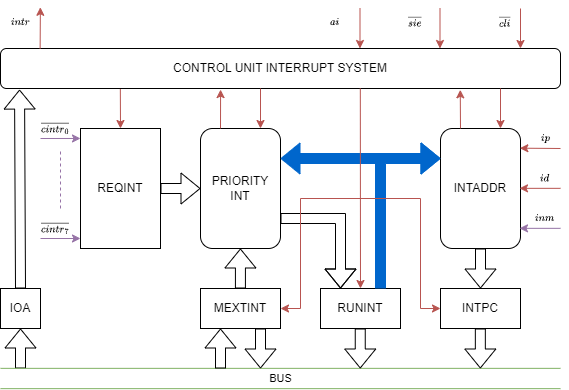
\includegraphics[width=0.8\textwidth]{media/isarchitecture.png}
    \end{figure}
\end{frame}

\begin{frame}
    \frametitle{Architecture Signals}
    \begin{itemize}
        \item $ip$ - Software Interrupt
        \item $id$ - ALU Overflow Interrupt
        \item $inm$ - external non-maskable interrupt (comes from $cinm$)
        \item $cintr_{i}$ - external maskable interrupt from device $i$
        \item $ai$ - external maskable interrupt active
        \item $intr$ - external maskable interrupt request to CPU
        \item $sie$/$cie$ - enable/disable external maskable interrupts
    \end{itemize}
\end{frame}

\begin{frame}
    \frametitle{Architecture Components}
    \begin{itemize}
        \item \texttt{REQINT} - Request external maskable interrupt register ($REQINT_{i} = 1$ means that the interrupt $i$ is requested)
        \item \texttt{MEXTINT} - Maskable external interrupt register ($MEXTINT_{i} = 1$ means that the interrupt $i$ is masked)
        \item \texttt{RUNINT} - Current running interrupts register ($RUNINT_{i} = 1$ means that the interrupt on level $i$ is running)
        \item \texttt{Priorrity INT} - Compute if the current interrupt has higher priority than the current running interrupt
        \item \texttt{INTADDR} - Compute the address of the ISR
        \item \texttt{INTPC} - The address for the current ISR
    \end{itemize}
\end{frame}

\begin{frame}
    \frametitle{External maskable interrupts Handling}
    \begin{enumerate}
        \item Verify for external maskable interrupt requests in the \texttt{REQINT} register.
        \item If there is one, verify if external maskable interrupts are enabled. (flag \texttt{I} in FR)
        \item If yes, filter the interrupts that are masked in the \texttt{MEXTINT} register.
        \item Find the highest priority interrupt that is not masked.
        \item Verify if it has higher priority than the current running interrupts in the \texttt{RUNINT} register:
        \item Send the interrupt to the CPU through the $intr$ signal.
        \item Wait for the CPU to acknowledge the interrupt. ($ai$ signal)
        \item Set the bit in the \texttt{RUNINT} register.
        \item Clear the bit in the \texttt{REQINT} register.
        \item Compute the address of the ISR and set the \texttt{INTPC} register.
    \end{enumerate}
\end{frame}

\begin{frame}
    \frametitle{External non-maskable interrupts Handling}
    \begin{enumerate}
        \item Verify for external non-maskable interrupt requests in the \texttt{inm} signal.
        \item Verify if there is no higher priority interrupt running.
        \item Compute the address of the ISR and set the \texttt{INTPC} register.
    \end{enumerate}
\end{frame}

\begin{frame}
    \frametitle{ALU Overflow Handling}
    \begin{enumerate}
        \item Verify for ALU overflow interrupt requests in the \texttt{id} signal.
        \item Verify if there is no higher priority interrupt running.
        \item Compute the address of the ISR and set the \texttt{INTPC} register.
        \item Inside the ISR, the CPU must clear the  overflow flag in the FR.
    \end{enumerate}
\end{frame}

\begin{frame}
    \frametitle{Software interrupts Handling}
    \begin{enumerate}
        \item Verify for software interrupt requests in the \texttt{ip} signal.
        \item There is no higher priority interrupt running.
        \item Compute the address of the ISR and set the \texttt{INTPC} register.
    \end{enumerate}
\end{frame}

\begin{frame}
    \frametitle{CPU acknowledge interrupts}
    \begin{enumerate}
        \item Save FR on the stack.
        \item Disable external maskable interrupts. (\texttt{EI} can be used to enable them back inside ISR)
        \item Save the current PC on the stack.
        \item Run the jump instruction from the \texttt{INTPC} register address.
    \end{enumerate}
\end{frame}

% \begin{frame}
%     \frametitle{Exam Questions}
%     Template: Having the following values in the registers at time 0,
%     interrupts requested with the time of the request and the type of the interrupt,
%     and how much time the CPU will take to handle every type of interrupt,
%     which is the order of the interrupts that will be handled by the CPU?
% \end{frame}


% \begin{frame}
%     \frametitle{Exam Questions}
%     \begin{table}[]
%         \begin{tabular}{|c|c|c|c|}
%             \hline
%             \texttt{REQINT} & \texttt{MEXTINT} & \texttt{RUNINT} & \texttt{FR} \\ \hline
%             0x00 & 0x00 & 0x00 & 0x00 \\ \hline
%         \end{tabular}
%     \end{table}

%     \begin{table}[]
%         \begin{tabular}{|c|c|c|c|}
%             \hline
%             Cycles from time 0 & Type of Request & Name \\ \hline
%             10 & External Maskable Interupt Level 5 & A \\ \hline
%             30 & External Maskable Interupt Level 3 & B \\ \hline
%             50 & External Maskable Interupt Level 7 & C \\ \hline
%             60 & External Maskable Interupt Level 1 & D \\ \hline
%             100 & External Non-Maskable Interupt & E \\ \hline
%             140 & ALU Overflow & F \\ \hline
%             150 & Software Interupt & G \\ \hline
%         \end{tabular}
%     \end{table}
% \end{frame}



% \begin{frame}
%     \frametitle{Exam Questions}
%     \begin{table}
%         \begin{tabular}{|c|c|c|c|}
%             \hline
%             Type of Request & Cycle to handle \\ \hline
%             External Maskable Interupt Level 0 & 30 \\ \hline
%             External Maskable Interupt Level 1 & 20 \\ \hline
%             External Maskable Interupt Level 2 & 10 \\ \hline
%             External Maskable Interupt Level 3 & 40 \\ \hline
%             External Maskable Interupt Level 4 & 20 \\ \hline
%             External Maskable Interupt Level 5 & 30 \\ \hline
%             External Maskable Interupt Level 6 & 10 \\ \hline
%             External Maskable Interupt Level 7 & 20 \\ \hline
%             External Non-Maskable Interupt & 5 \\ \hline
%             ALU Overflow & 10 \\ \hline
%             Software Interupt & 10 \\ \hline
%         \end{tabular}
%     \end{table}
% \end{frame}



% \begin{frame}
%     \frametitle{Exam Questions}
% \end{frame}

\section{UART}

\begin{frame}
    \frametitle{Introduction to UART}
    \begin{itemize}
        \item Universal Asynchronous Receiver-Transmitter.
        \item Hardware communication protocol.
        \item Used for asynchronous serial communication.
    \end{itemize}
\end{frame}

\begin{frame}
    \frametitle{Setting Up UART}
    \begin{itemize}
        \item Two devices connected by TX and RX lines.
        \item Voltage levels must match. (3.3 V, 5 V)
        \item Baud rate must be agreed upon. (9600, 19200, 38400, 57600, and 115200)
        \item Data format must be agreed upon. (8E1, 8 data bits, even parity, 1 stop bit)
        \item Flow control:
        \begin{itemize}
            \item Hardware: RTS/CTS (Request to Send/Clear to Send)
            \item Software: XON/XOFF (ASCII characters 0x11 and 0x13, ready to accept data as receiver)
            \item No flow control
        \end{itemize}
    \end{itemize}
\end{frame}

\begin{frame}
    \frametitle{Format of UART Data}
    \begin{figure}
        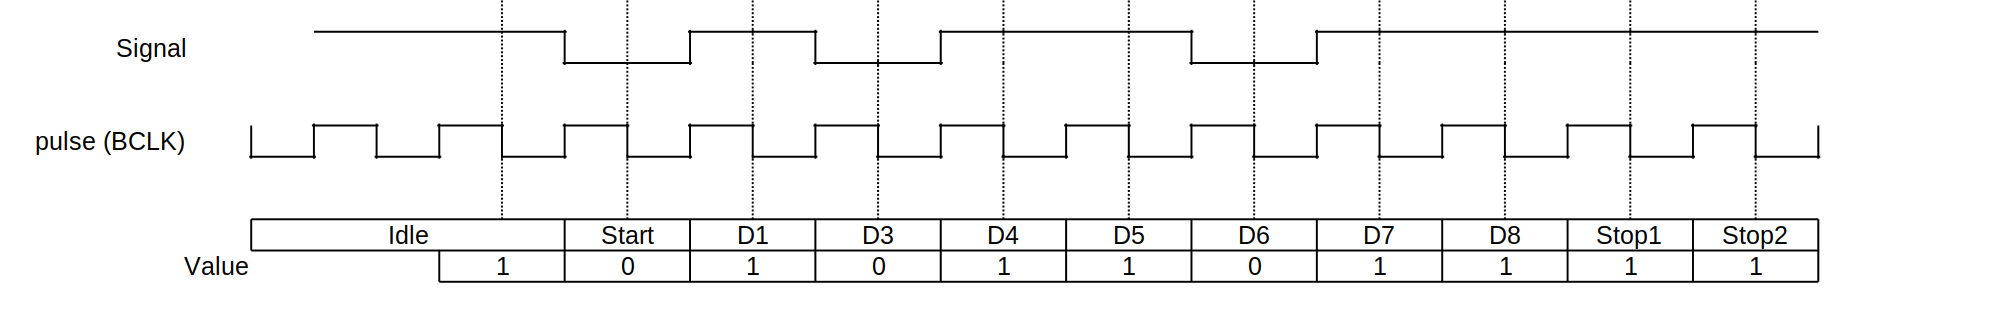
\includegraphics[width=0.9\linewidth]{media/UART.png}
        \caption{By EidenNor - Own work, CC BY-SA 4.0, https://commons.wikimedia.org/w/index.php?curid=118379174}
    \end{figure}
\end{frame}

\begin{frame}
    \frametitle{Transmission of Data Bits}
    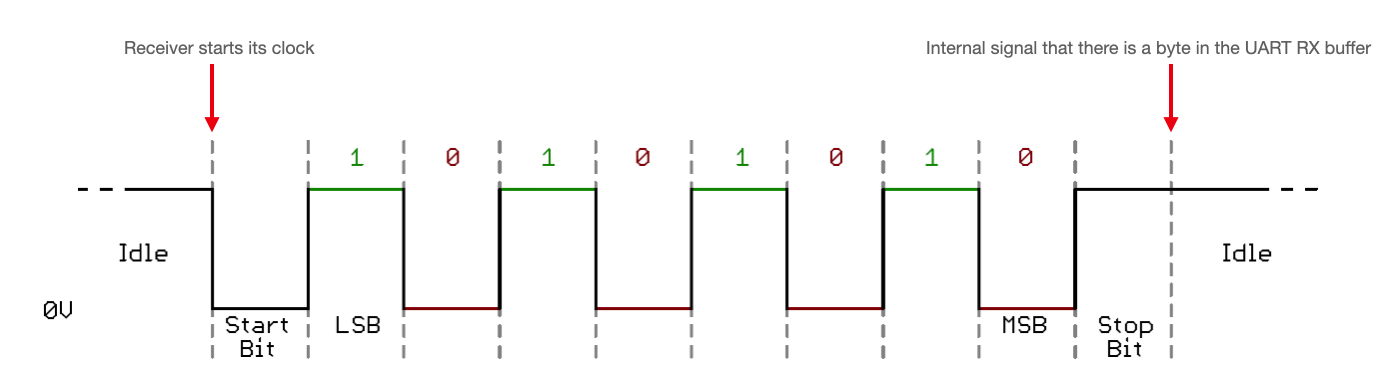
\includegraphics[width=0.8\linewidth]{media/uart_timing.png}
\end{frame}


\begin{frame}
    \frametitle{Exam Question}
    Template: Having the X UART configuration, what is the maxim data rate that can be achieved?

    Example: Having the 3.3V 9600 baud rate 8E1 with no flow control UART configuration, what is the maxim data rate that can be achieved?
\end{frame}


\section{Q\&A}
\begin{frame}
\end{frame}

%\begin{frame}
%\frametitle{Table of Contents}
%\tableofcontents
%\end{frame}


\end{document}